%!TEX options = --shell-escape


\documentclass[bachelor]{thesis-uestc}

\title{全路网智能路径规划}
\author{董林森}
\advisor{郭宏亮\chinesespace 副教授}
\school{自动化工程学院}
\major{测控技术与仪器}
\studentid{2014070906006}

\begin{document}

% \makecover[0]

% this is a thesis template with mutiple files: the chapters and the misc in standalone mode
% to avoid too many files in current folder, template add extra direcotry: chapter and misc
% please do not change the sequence of each one except the chapters themselves.
% by FengYouzheng.

% abstract
\documentclass{standalone}
% preamble: usepackage, etc.
\begin{document}
	
\begin{chineseabstract}
随着人工智能和机器学习的快速发展,强化学习,作为一个该领域的一个重要分支,展现它在很多领域的应用潜力,比如围棋。作为一个决策和控制的框架,强化学习同样可以被应用在路径规划系统,而后者被广泛应用于车辆导航等系统。在我们的工作中,我们尝试使用强化学习解决路径规划问题,并且解决了多个不同的路径规划场景问题,特别是解决了一些传统的基于搜索的路径规划算法,比如 A star,dijkstra 等不能解决的场景。

论文分为三个部分

\chinesekeyword{强化学习,路径规划}
\end{chineseabstract}

\end{document}
\documentclass{standalone}
% preamble: usepackage, etc.
\begin{document}

\begin{englishabstract}

	In a transportation system, giving the optimal path given the start point and target point is wildly used in many real world application. These kind of algorithms were called route planning algorithms or shortest path algorithms. As the transportation network getting more complicated and transportation tools developing rapidly such as subway, bus and airlines, traditional routing algorithms based on static map are no longer suitable for current environment. So it becomes a key research field that how to develop more strong and flexible routing algorithm that can be meet the new requirements.

    With the development of Artificial Intelligence and Machine Learning, Reinforcement Learning (RL), as an important method in this field, have showed its great potential in field like Go. As a decision-making and control schema, RL also can be applied in route planning system. In our work, we applied RL to route planning problem and solved various scenarios, especially for the scenario that traditional search-based route planning algorithms like $A^*$, $Dijkstra$ can't solve.
    
    % The content of the dissertation is divided into five parts. In section one, we give the mathematical formulation of route planning problem, meanwhile we put forward some variations based on basic route planning problem like by adding extra turning cost, electrical car routing with moving distance limitation and charging sites, dynamics map involved traffic jam etc. In section two, we introduce the search-based routing algorithm like $A^*$, $Dijkstra$, and some variations based on these to solve some specific scenarios mentioned above. Then we give a simple analysis about the shortcoming of these methods, such as lacking flexibility, can't solve dynamics environment or more complicated users' requirements. In section three, we give the background of RL, including the Agent-based modeling, controlling schema based on Markov Decision Process (MDP). Also we give some basic concepts within RL like value function, policy function, at last we focus on value-based methods which we will use for route planning problem. In section four, we will focus on introduction our method, firstly, we adapt route planning problem into a standard MPD problem, and for each scenario, we give a RL algorithm based on $Q-learning$. In section five, we give the implementation of the code and experiments results. At last, we conclude our work and propose the future work.
  
	\englishkeyword{reinforcement learning, route planning, $Q-learning$, $Dijkstra$, $A^*$, turning cost, electrical car routing problem, dynamics map}
\end{englishabstract}

\end{document}

% table of contents
\thesistableofcontents

% thesis contents
\documentclass{standalone}
% preamble: usepackage, etc.
\begin{document}

\thesischapterexordium

\section{研究工作的背景与意义}
随着城市交通网络的发展和交通工具的进步,针对路径规划问题设计的各种系统和算法逐渐在现实生活中被广泛的应用,比如在日常驾驶出行或乘坐公共交通等情景中,人们越来越频繁的使用这一功能。同时随着交通网络复杂度提高,规模增大,多种交通工具的出现以及城市堵车给城市交通网络带来的随机性和动态性,这给传统的路径规划问题带来了全面的挑战。同样,随着自动驾驶技术的发展,路径规划问题作为自动驾驶的导航模块中重要的部分同样扮演者不可或缺的角色。因此如何更好的设计出更强大,更具灵活性的,更高效的路径规划算法具有重要的发展意义,而这也成为了当前各国学者的研究热点之一。

% \footnote{脚注序号“\ding{172},……,\ding{180}”的字体是“正文”,不是“上标”,序号与脚注内容文字之间空1个半角字符,脚注的段落格式为:单倍行距,段前空0磅,段后空0磅,悬挂缩进1.5字符;中文用宋体,字号为小五号,英文和数字用Times New Roman字体,字号为9磅;中英文混排时,所有标点符号(例如逗号“,”、括号“()”等)一律使用中文输入状态下的标点符号,但小数点采用英文状态下的样式“.”。}

\section{路径规划问题的国内外研究历史与现状}
路径规划问题,最早被转换为图论中的最短路径问题,最短路径问题根据图的类型不同,分为无向图上的最短路径、有向图上的最短路径、单源最短路,多源最短路等等。Edsger W. Dijkstra 最早于1956年,提出了著名的 $Dijkstra$ 算法,给出了单源最短路算法,随后包括 $Bellman-Ford$, $A^* search$, $Floyd-Warshall$ $Johnson's algorithm$, $Viterbi algorithm$等被相继提出,在一定程度上都降低了最短路算法的时空复杂度。\par
但随着交通环境复杂度的增加(大陆级别的地图范围)和用户需求的增加(例如需要考虑多种交通工具的组合,倾向选择公共交通方式,选择非收费路段等),先前提出的基于静态网络和单一的度量方法都已经无法适应。因此各国学者和研究机构,例如Microsoft,Karlsruhe Institute of Technology等针对不同的场景,提出了改进的算法。

\section{本文的主要贡献与创新}
我们的主要贡献包括:1)首次将端到端的强化学习应用到了路径规划算法,并证明了其可用性。2)使用强化学习解决了传统算法难以解决的某些路径规划场景。

\section{本论文的结构安排}
本文的章节结构安排如下:\par
论文分为五个部分,在第一章,我们给出了路径规划问题的基本数学形式,同时我们给出了几种基于基本路径规划问题的变形,例如带有额外转弯惩罚的路径规划问题,带有行驶长度限制的电动车路径规划问题,以及动态地图环境下的路径规划。这些特殊的场景是传统的最短路径算法所难以解决的,我们将通过强化学习的方法很好的解决这些场景;在第二章,我们先给出传统的基于搜索的路径规划算法,例如 $A^{*}$,$Dijkstra$ 等,并给出为了解决以上特殊场景而做出的一些改进算法。同时我们试着简单分析这类方法的缺点,例如不够灵活,无法应对复杂动态环境或更复杂的用户需求等;在第三章,我们给出强化学习的基本概念和相关方法,包括了强化学习的基于智能体建模的方法和基于马尔科夫决策过程的控制结构。以及强化学习中的基本概念,如价值函数,策略函数等,最后着重介绍为了解决路径规划问题使用的基于值函数的方法;在第四章,我们将介绍我们的方法,首先将路径规划问题表述为一个标准的马尔科夫决策过程,然后针对不同的环境,我们设计了基于 $Q-learning$ 的强化学习算法。在第五章,我们给出了具体的代码实现方法和实验结果;最后给出全文的总结和未来的研究方向。

\end{document}
\documentclass{standalone}
% preamble: usepackage, etc.
\usepackage{tikz}
\usepackage{amsmath}

\begin{document}

\chapter{路径规划问题}
在这一章,我们引入路径规划问题,给出其严格的数学定义。然后介绍随着现实交通网络的复杂化,路径规划问题所出现的新的形式和挑战,并给出其数学形式。通过这一章,我们将详细阐述我们的工作所解决的问题,这将有利于在随后的相关章节中强化学习算法的设计和实验。
\section{路径规划问题的数学形式}
路径规划问题,如绪论1.2节所述,根据问题建模形式,其算法分为基于图的搜索算法和基于采样的规划方法。在本文中,我们使用基于图的搜索算法,然后给出其相应的数学形式。\par
令 $v\in \{1,2,3...n\}$表示图中的某个顶点,假设有$n$个顶点。令$e_{i,j}$表示图中的一条从点$i$到点$j$的一条边,假设共有$m$条边。令$V$ 表示图中节点的集合,令$E=\{e_{i,j})| i,j \in V \}$表示图中边的集合。
令$f:E \to \mathbb{R}$ 表示为一个将图中的任意一条边映射到某一实数集上的函数,在静态的最短路径问题中,该函数一般等价于路径长度,但在本文中,为了使模型和算法应用于多种场景中,我们将其定义为抽象的损失函数,即通过某条边的损失,以使得定义能够适应于复杂的路径规划场景。$f$函数的输入包括但不限于某条边,在不同问题中,可能会有额外的输入信息以计算该函数值,例如在带有转弯额外惩罚的场景中,车辆是否转弯也作为函数的输入以计算损失值。则由以上定义可得一个有向图定义为$G=(V, E, f)$,其包含一个点集$V$,一个边集$E$和一个损失函数$f$。

我们定义$P=\{v_1, v_2,...,v_k\}$为图中的一条路径,路径的长度或总损失定义为$L(P) = \sum_{i=1}^{j-1} f(e_{v_i,v_{i+1}})$。基于以上定义,最短路径规划问题可以被定义为:在图$G$中,给定某一起始点$v_s$和终止点$v_t$,找到某一条路径$P_{optimal}$使得$L(P_{optimal})$最小,公式定义如式\ref{optimalpath},其中 $v_s$为路径$P$的起点,$v_t$ 为路径$P$的终点,argmin($\cdot$)为取最小值参数的函数。
\begin{equation}
\label{optimalpath}
P_{optimal}(v_s, v_t) = argmin_{P}(L(P(v_s, v_t)))
\end{equation}
一个简单的实例如图\ref{fig2shortest}所示,标注深色的边表示了从节点 A 到节点 F 的最短路径。
\begin{figure}[H]
    \centering
	\includegraphics[width=7.0cm]{pic/2-1.pdf}
	\caption{最短路径求解示例}
	\label{fig2shortest}
\end{figure}

\section{不同场景及其数学形式}
在这一章节,我们将介绍基于2.1章节的基本最短路径问题形式的几个特殊场景,这些场景是由于随着现代交通网路的发展和复杂化,以及交通工具的扩展而出现的一些不同于传统形式的特殊场景。这些场景的出现使得我们需要对原有的问题形式进行一定的修改和重新定义,以方便我们进行相应算法的设计和实现。在本章节中将要介绍的场景也是我们将要使用强化学习进行应用和解决的场景。通过给出其数学形式上的严格定义,有助于我们在随后进行基于马尔科夫决策过程的建模和强化学习算法的设计。

\subsection{场景1:简单网格地图}
第一个场景为简单网格地图场景,设计该场景的原因在于,我们将通过这一简单的场景验证强化学习模型在路径规划问题上的可用性。在该场景中,我们通过一个二维网格表示地图,在任意一个点,在不越过地图界限的情况下,车辆可以向上下左右四个方向移动,如图\ref{figcase1}所示。令 $N$ 表示图的行数, $M$表示图的列数,左下角点的坐标为$(0,0)$,右上角的坐标为$(N-1, M-1)$。在图中,我们定义$S$ 为起点,$E$为目标点,某一时刻,车辆所处的位置由图中的$car$ 点表示。车辆在移动过程中,其每次移动距离为一个格子,边上的损失函数 定义为式\ref{costfunc},其中$C\in\mathbb{R}$, $C\ge0$,且$C$为常数。
\begin{equation}
\label{costfunc}
    f(e_{v_i,v_{i+1}}) = C 
\end{equation}
\begin{figure}[h]
\centering
    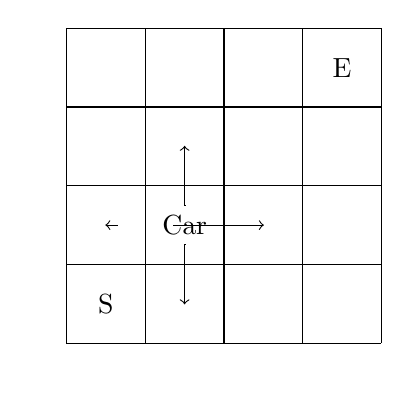
\begin{tikzpicture}[every node/.style={minimum size=1cm-\pgflinewidth, outer sep=0pt}, arrow/.style={thick}]
        \draw[step=1cm,color=black] (-2,-2) grid (2,2); 
        \node[](start) at (-1.5, -1.5) {S};
        \node[](end) at (1.5, 1.5) {E};
        \node[](car) at (-0.5, -0.5) {Car};
        
        \node[](car_up_center) at (0.0, -0.25) {};    
        \node[](car_up) at (-0.5, 1.0) {};
        
        \node[](car_down_center) at (0.0, -0.75) {};
        \node[](car_down) at (-0.5, -2.0){};
    
        \node[](car_left_center) at (-1.35, -0.5) {};
        \node[](car_left) at (-2.0, -0.5){};
    
        \node[](car_right_center) at (-0.65, -0.5) {};
        \node[](car_right) at (1.0, -0.5){};
        
        % \node[](charge site) at (-0.5, 1.5) {$t_{1}$};
        % \node[](charge site) at (1.5, -0.5) {$t_{2}$};
        \draw[->, to path={-| (\tikztotarget)}]
     	( car_up_center) edge (car_up)  (car_down_center) edge (car_down) ;
         \draw[<-, to path={-| (\tikztotarget)}]
     	(car_left) edge (car_left_center) (car_right) edge (car_right_center);
    \end{tikzpicture}
    \caption{场景1:简单网格地图}
    \label{figcase1}
\end{figure}

\subsection{场景2:带有转弯惩罚的场景}
在现实交通网络中,对最短路径计算结果具有重要影响的因素之一为转弯方向的选择,例如在图\ref{figcase1}实例中,同时存在多条从起点到终点的最短路径,但在实际交通网络中,例如中国等靠右行驶的国家中,左转往往比直行和右转具有更长的时间消耗。因此在两条最短路径行驶长度完全相同的情况下,较少左转的路径往往实际消耗的时间更少。
我们通过加入额外的转弯惩罚设计了场景2,在该场景中,在任意一条边上的移动损失函数定义为式\ref{case2movingcost},其中$A \in\mathbb{R}, C\ge0$为常数,表示转弯的额外惩罚。
\begin{equation}
\label{case2movingcost}
f(e_{v_i,v_{i+1}}) = \begin{cases}
C + A &\mbox{if car turn left or turn around}\\
C &\mbox{else}
\end{cases}
\end{equation}

\subsection{场景3:带有行驶路径限制和充电桩的场景}
随着电动汽车的普及和推广,基于电动车的路径规划也作为某一特定问题被各国学者进行研究。该场景的特殊性在于,电动车普遍行驶距离较短,在进行单次路径规划中,我们在求解最短路径的同时,需要保证其在任意行驶过程中保持电量大于零,如果电量过低,需要到就近的充电桩进行充电后再行驶。
这给原始的简单网格地图的场景带来了如下变化。\par
首先,地图中增加多个充电桩的位置,充电桩的集合被定义为 $T = \{t_{1}, t_{2}...,t_{k}\}, t_i \in V$;
同时对车辆,除去其当前位置,我们需要引入$\mathrm{power}\in[0, FULL\_POWER]$表示车辆当前剩余电量。其中 $FULL\_POWER\ge0$,表示车辆电量的最大值。修改后的地图如图\ref{figcase2}所示

\begin{figure}[H]
\centering
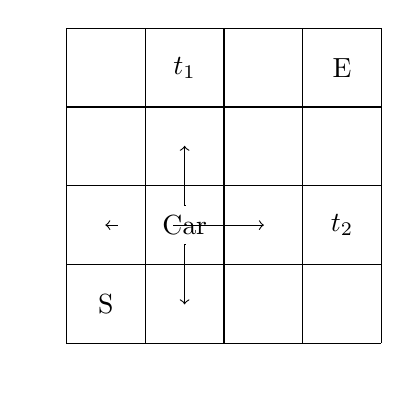
\begin{tikzpicture}[every node/.style={minimum size=1cm-\pgflinewidth, outer sep=0pt}, arrow/.style={thick}]
    \draw[step=1cm,color=black] (-2,-2) grid (2,2); 
    \node[](start) at (-1.5, -1.5) {S};
    \node[](end) at (1.5, 1.5) {E};
    \node[](car) at (-0.5, -0.5) {Car};
    
    \node[](car_up_center) at (0.0, -0.25) {};    
    \node[](car_up) at (-0.5, 1.0) {};
    
    \node[](car_down_center) at (0.0, -0.75) {};
    \node[](car_down) at (-0.5, -2.0){};

    \node[](car_left_center) at (-1.35, -0.5) {};
    \node[](car_left) at (-2.0, -0.5){};

    \node[](car_right_center) at (-0.65, -0.5) {};
    \node[](car_right) at (1.0, -0.5){};
    
    \node[](charge site) at (-0.5, 1.5) {$t_{1}$};
    \node[](charge site) at (1.5, -0.5) {$t_{2}$};
    \draw[->, to path={-| (\tikztotarget)}]
 	( car_up_center) edge (car_up)  (car_down_center) edge (car_down) ;
     \draw[<-, to path={-| (\tikztotarget)}]
 	(car_left) edge (car_left_center) (car_right) edge (car_right_center);
\end{tikzpicture}
\caption{场景3:电动车路径规划问题的网格地图}
\label{figcase2}
\end{figure}
\section{现有的基于搜索的算法}
\subsection{Dijkstra 算法}
Dijkstrea 算法由荷兰计算机科学家 Edsger Wybe Dijkstra在1956年提出的单源最短路径算法,在随后的几年内被正式发表\citing{Dijkstra}。
\subsubsection{算法描述}
首先定义我们起始的点为$v_s$,令$D_{v_j}$表示点$v_j$到初始点 $v_s$的距离。Dijkstra 算法首先赋予一些初始距离值,然后通过迭代计算和优化距离值,算法的基本流程如下。\par
第一步,首先将所有点标记为未访问过,并放入一个未访问的点的集合$Q$中,然后对初始点,设置它的距离值$D$为0,剩余点设置为无穷大。
第二步,从未访问集合$Q$中取出具有最小距离值的点,查询它的邻居节点的距离值,
如果邻居节点通过当前节点后其距离值降低,则更新邻居节点的距离值,这一步操作成为松弛操作。当前节点的所有邻居都被更新后,将当前节点标记为已访问,然后重复第二步,直到未访问集合为空。
第三步,如果目标节点被标记为已访问,则表示我们找到了一条从起点到目标节点的最短路径。
在计算过程中,我们可以对每个点维护一个前驱节点值,即当前节点的距离值被某个邻居节点的距离值更新时,同时更新该前驱值为对应邻居节点。在计算结束后,可以通过该前驱节点值递归的输出最短路径。
\subsubsection{复杂度分析}
Dijkstra 算法的时间复杂度上下界可使用大$O$符号,由用点集$V$和边集$E$组成的函数表示,时间复杂度的上下界的紧致程度或长数值大小由算法中$Q$集合的实现决定。Dijkstra复杂度为$O(|V|^2)$,其中$|V|$为图中点的数量。但一个更精确的表述为 $O(|E|\cdot T_{dk} + |V|\cdot T_{em})$,其中$T_{dk}$表示完成集合中键的降序排列时间复杂度,$T_{em}$表示从集合中取出最小键值的时间复杂度。
\subsubsection{Dijkstra的相关改进算法}
在 Dijkstra 算法被提出后,许多基于 Dijkstra 的优化算法被提出。
由于在 Dijkstra 算法中很重要的一步为从$Q$集合中取出具有最小距离值$D$的节点,因此Boas等人提出了基于优先队列实现的改进算法,使得其复杂度降到了$O(|V|loglog|V|)$。
Fredman和 Tarjan通过斐波那契堆实现的算法复杂度为$O(|E| + |V|log|V|)$\citing{Fredman1984Fibonacci}。
\subsection{Floyd 算法}
Floyd 算法为 Robert Floyd 在1962年提出\citing{Floyd1962Algorithm},同年代,Warshall 也提出了类似算法,因此该算法又被称为 Floyd-Warshall 算法。Floyd 解决了多源最短路问题,其时间复杂度为$O(|V|^3)$,它通过枚举任意两点之间可能的最短路径然后按照基于动态规划的思想进行更新。
\subsubsection{算法描述}
设$D_{i,j,k}$表示从顶点$i$ 到顶点$j$的只以$(1..k)$集合中的节点为中间节点的最短路径长度,那么我们可以通过枚举$k \in \{1..|V|\}$,按照如下公式更新$D_{i,j,k}$:\begin{equation}
    D_{i,j,k} = min(D_{i,j,k-1}, D_{i,k,k-1} + D_{k,j,k-1})
\end{equation}

\subsection{Bellman-Ford 算法}
Dijkstra和 Floyd 算法存在的问题在于无法处理带有负环的图的最短路径问题,即如果在给定的图中,如果存在一个环路,通过该环路的损失为负值,那么理论上可以无限的降低总损失值,因而无法给出正确的最短路径。所以Richard Bellman 和 Lester Ford于1958年年提出了可以处理负环的 Bellman-Ford 算法\citing{Bellman1958On}。
\subsubsection{算法描述}
与 Dijkstra 算法类似,Bellman-Ford也是基于松弛操作,然而 Dijkstra 是通过贪心的选择距离最小的点进行松弛操作,而后者是简单的通过枚举边然后对边上的两个端点进行松弛操作,这一过程共进行$|V|-1$次,由于任意一个图上的最短路径长度不会超过$|V|-1$。
因此在$|V|-1$次松弛操作后,理论上保证了在解存在情况下,算法能够找到最短路径的解。最后 Bellman-Ford 算法通过第$|V|$次松弛操作,检测是否存在负环,如果在第$|V|$次松弛操作时,仍然存在可被缩小的距离值,那么说明负环存在。
\subsection{$A^{*}$ 算法}
$A^{*}$ 算法是一类重要的启发式搜索算法\citing{Astar},它的核心思想在于,通过对搜索的状态空间中的每一个搜索位置按照某一启发式函数进行评估,选择具有最优值的搜索点进行下一步搜索。
由于路径规划问题本质上一个在图上的搜索问题,因此$A^{*}$ 算法也被应用到了该问题中。
\subsubsection{算法描述}
在$A^{*}$ 算法中,最重要的为设计启发式函数$f(v_i)$,或者成为估算函数。一般函数具有$f(v_i) = g(v_i) + h(v_i)$的形式,其中$g(v_i)$表示从初始点走到 $v_i$的代价值,$h(v_i)$表示从点$v_i$到目标点的估计距离。在实际的算法中,我们会维护关于$g(v_i)$的表,对于$h(v_i)$,我们一般使用欧几里得距离,曼哈顿距离或切比雪夫距离等计算方法作为估算函数。\par
算法的基本流程如下,首先定义集合$C_{set}$为被估算的节点集合,$O_{set}$为将要被估算的节点集合,初始时只包括起点。起点的 $g$函数值为0,$h$函数值设为某一距离函数下的计算结果。当$O_{set}$不为空时,我们取出其中$f$值最小的点$v_{min}$,枚举该点的邻居$v_{neighbor_i}$,如果该点不在$C_{set}$中,根据松弛操作判断$v_{neighbor_i}$的$g$值是否在通过$v_{min}$后更小,如果是,则更新$v_{neighbor_i}$的$g, h, f$值,同时将$v_{neighbor_i}$加入$O_{set}$,如果否,则不做任何更新和操作。最终当我们取出的点$v_{min}$为目标点时,说明我们找到了解。
\subsubsection{复杂度分析}
$A^{*}$ 算法的复杂度依赖于启发式函数的设计。在最坏情况下,$A^{*}$的复杂度相当于一个不带任何优化和限制的搜索算法的复杂度 $O(b^d)$,其中$b$为状态空间的宽度,即每个搜索状态的后继状态的平均数量,在该问题中为每个节点相临节点的数量,$d$为搜索空间的深度,在该问题中为路径的长度的最大值,即为定点的个数。而一个好的启发式函数可以大大减少搜索状态的数量,特别是$b$的值。作为搜索算法,复杂度的定义显然与搜索节点的数量成正比,因此我们定义 $N$: 
    \begin{equation}
        N + 1 = 1 + b^* + (b^*)^2 + ... + (b^*)^d
    \end{equation}
而最优的启发式函数$h_*(x)$具有$b=1$。对于任意一个非最优的启发式函数,当其启发式函数符合方程\ref{eq3astar},其时间复杂度为多项式级别。
    \begin{equation}
    \label{eq3astar}
        |h(x) - h_*(x)| = O(logh_*(x))
    \end{equation}
\subsection{改进算法}
随着交通网络的复杂度提高,基于图的搜索算法难以处理过大的地图,因此一些优化方法便被提出。\par
Thorup 和 Zwick 提出了基于预处理和查询的分步方法\citing{Thorup2001Compact}。这类方法首先离线对原始图进行预处理,降低原问题的复杂度,然后在查询阶段,利用预处理阶段得到的数据和简化后的图快速给出路径规划结果。
第二类改进算法为结构化的最短路径算法,交通网络本身具有一定的结构性质,即分层模型,通过将地图按照一定的规则分层,然后对分层后的模型做路径规划可以提升原有算法的性能。例如 Sanders 和 Schultes 提出了通过定义邻近集合和邻近搜索的方法\citing{Sanders2005Highway, Sanders2006Engineering},这类方法被称为公路结构化方法(Highway Hierarchies)方法。同样 Geisberger 等人提出了基于缩点的结构化方法\citing{Geisberger2008Contraction},通过对节点按照重要性排序,然后将非重要的节点进行缩点和替换从而减小图的规模。\par
Delling等人提出了可定制化的最短路径算法\citing{Delling2011Customizable},他们将图分为静态的拓扑结构,包括了边,节点等,和计算模式,即如何计算行驶损失的方法两部分。使得前者维持静态,后者为一个动态模块。该算法分为三个步骤,首先为独立损失计算部分,在这一步只对静态图进行预处理,第二步为定制化计算损失阶段,对不同的损失计算方法进行处理。最后为查询阶段,根据不同的损失计算方法给出结构。

\section{本章小结}
作为本文的正式内容的第一个章节,我们给出了路径规划问题的定义,以及出现的多个新的场景和需求。通过给出严格定义,将为下面章节我们使用强化学习解决问题提供较严格的数学形式支持。同时给出了传统的基于图的搜索算法,包括经典的 Dijkstra 算法和近些年各国学者提出的种种改进算法,但我们也看到了这些算法存在的部分问题。现有的算法,大多是基于不同场景的定制化算法,对于不同的最短路计算函数,需要单独设计不同的算法,这导致不同场景下的算法具有较少的通用性和可扩展性。其次随着交通场景的复杂化和规模增大,现有的改进算法大多基于较为简单的预处理来增加额外的信息和降低图的规模。因此我们将尝试使用强化学习解决这些问题,并为路径规划问题未来的设计和发展提供新的思路。
\end{document}
\documentclass{standalone}
% preamble: usepackage, etc.
\begin{document}

\chapter{基于搜索的路径规划方法}
\section{Dijkstra 算法}
\section{$A^{*}$ 算法}
\section{相关改进算法}
\end{document}
\documentclass{standalone}
% preamble: usepackage, etc.
\begin{document}

\chapter{强化学习基础}

强化学习是一种学习如何进行控制和决策的框架,强化学习的灵感来自于仿生学,它完成了从当前的环境状况到行为的映射,并通过学习这一映射过程使得从环境中得到的奖赏值最大化。这样一种框架被誉为可能是发展为强人工智能的框架,包括博弈论、控制理论、群体智能、多智能体系统等领域都与强化学习可以进行结合和交叉。在控制领域,强化学习被视为一种拟合动态规划方法。在博弈论领域,它被用来解释均衡点的出现及其原因。它和有监督学习,无监督学习组成了机器学习领域三个基本的学习框架。它不同于有监督学习和无监督学习,原因在于,在强化学习中,并不存在类似于有监督学习中的标签信息,只有奖赏信号用于指导整个学习过程,同样这也不同于无监督学习中没有任何信号和标签指导学习过程。\par

\section{智能体建模方法和马尔科夫决策过程}
\subsection{智能体建模方法}
强化学习框架的设计一般基于智能体建模的方式实现,基于智能体的模型是一种为了模拟控制和交互的计算模型,这样一种框架包括智能体和环境两类主体,其在多个领域都有广泛的应用,如在生物学中用于研究种群的分布,人口变化等问题,在经济和社会学中,用于研究城市人口流动和城市规划问题,消费者行为分析等。在强化学习中,我们通过图4-1所示的框架对强化学习进行建模。Agent 表示智能体,即表示我们的控制算法的主体。Environment 表示环境,智能体与环境进行交互。在路径规划问题中,智能体代表了我们的路径规划算法,它输出控制车辆的行为如直行,左转等,而环境代表了实际的地图环境,如我们在第2章节所述的多个场景等。
\begin{figure}[h]
	\includegraphics[width=12.0cm]{pic/4-1.png}
	\caption{强化学习框架}
	\label{4-1}
\end{figure}
\subsection{马尔科夫决策过程}
马尔科夫决策过程(Markov Decision Process, MPD)为建模决策问题提供了一个数学框架,MPD对于通过动态规划或强化学习解决和研究优化问题十分重要。这一框架最早于1950年提出,随后 Ronald A. Howard 在书中做了详细做了详细的研究。
在强化学习中,我们通常把环境规范到马尔科夫决策过程,这样的设计有利于强化学习算法的设计,同时便于算法的相关理论证明。\par
精确的来说,智能体和环境在一个离散的时间序列$t=0,1,2,3,... ..$上进行交互,在一个时刻$t$上,智能体接受到表示环境状态的信息(state),随后根据自己身的策略和决策系统,给出行为(action)。环境在接收到该行为后,依据某一概率转移矩阵,进行状态的更新,同时计算一个对应的奖赏信号(Reward),环境把新的状态和奖赏信号返回给智能体,此时进入下一个时刻,该过程不断重复直到环境返回一个结束信号。因此根据以上描述,我们定义一个马尔科夫决策过程是一个包含5个元素的元组,表示为$MDP=(S, A, P_{a}, R_{a}, \gamma)$,其中$S$为一个表示状态的有限集合。$A$表示一个行为的有限集合,更特别的用$A_s$表示某一状态$s$下的可取的行为的集合。$P_a(s, s') = \mathbb{P}(s_{t+1} = s'|s_t = s, a_t=a)$表示在$t$时刻,状态为$s$,采用行为$a$时,$s_{t+1}$为$s'$的概率。$R_a{s, s'}$表示在$t$时刻,状态为$s$,采用行为$a$,状态转移到$s'$时,环境的即时奖赏值。$\gamma \in [0, 1]$表示折扣因子,表示我们主观对即时奖赏和未来奖赏重要程度的差别。\par 

\section{强化学习}
强化学习的目标在于找到一个策略(Policy)使得在该策略下,智能体能够最大化其从环境中受到的累计奖赏值。因此在控制或者决策问题中,我们假设我们的目标或目的即为最大化累计奖赏,这一假设成为奖赏假设。而这一形式也是强化学习相比于其他机器学习框架独特所在。\par
策略定义为:$\pi(a|s) = \mathbb{P}[a_t=a | s_t=t]$,即策略为一个给定状态的行为的概率分布。策略完全定义了一个智能体的行为,同时其决策只依赖于当前时刻的状态。
因此在一个决策过程中,给定$MDP=(S, A, P_{a}, R_{a}, \gamma)$ 和$\pi$,智能体和环境进行交互,最终产生一条轨迹(Trajectory),定义为: $s_0, a_0, r_0, s_1, a_1, r_1, ...$。同样,如果我们得到的某条轨迹是采样直到收到了环境的终止信号,则成该轨迹为一个完整的节(Episode)。如前面所述,智能体的目标在于最大化累计奖赏,累计奖赏的定义如下:
\begin{center}
    \begin{equation}
        G_t=r_{t+1} + \gamma r_{t+2}+... = \sum_{k=0}^{\infty}\gamma^{k}R_{t+k+1}
    \end{equation}
\end{center}
\subsection{价值函数}
在这一节,我们将介绍强化学习中一个重要的函数,价值函数,它表示了对一个状态的好坏程度的估计值,好坏被严格定义为在该状态下未来期望值的大小。\par
状态价值函数$v_{\pi}(s)$表示以状态$s$作为初始状态,按照策略$\pi$进行决策下,智能体所受到的累计奖赏值。即:
\begin{center}
    \begin{equation}
        v_{\pi}(s) = \mathbb{E}_{\pi}[G_t|s_t=s] = \mathbb{E}[\sum_{k=0}^{\infty}{\gamma^k{R_{t+k+1}}}|s_t=s]
        \mbox{, for all s $\in$ S.}
    \end{equation}
\end{center}
其中$\mathbb{E[\cdot]}$表示给定策略$\pi$的一个随机变量的期望值。
\par
类似的,我们定义状态行为函数为$q_{\pi}(s,a)$表示以状态$s$作为初始状态,采取行为$a$,然后按照策略$\pi$进行决策下,智能体所受到的累计奖赏值。即:
\begin{center}
    \begin{equation}
        q_{\pi}(s,a) = \mathbb{E}_{\pi}[G_t|s_t=s, a_t=a] = \mathbb{E}[\sum_{k=0}^{\infty}{\gamma^k{R_{t+k+1}}}|s_t=s, a_t=a]
    \end{equation}
    
\end{center}
\subsection{最优策略和最优价值函数}
求解一个强化学习问题,意味着我们需要找到一个策略函数,使得其在决策过程中得到的累计奖赏值较大。而引入价值函数使得我们可以获得对策略的偏序关系。所以我们定义一个策略$\pi$比另一个策略$\pi'$更优,当且仅当其满足:$v_{\pi}{}s \geq v_{\pi'}(s), for all s \in S$。总是至少存在一个策略优于或等于其他策略,这个策略就是最优策略。定义最优策略为$\pi_{*}$,其对应的状态价值函数为$v_{*}(s)$,且有:
\begin{center}
    \begin{equation}
        v_{*}(s) = max_{\pi}v_{\pi}(s),
        \mbox{for all s $\in$ S.}
    \end{equation}
\end{center}
同样最优策略的对应状态行为函数也满足:
\begin{center}
    \begin{equation}
        q_{*}(s, a) = max_{\pi}q_{\pi}(s, a),
        \mbox{for all s $\in$ S and a $\in A_s$.}
    \end{equation}
\end{center}
\subsection{基于价值函数的控制方法}
在强化学习中,根据是否具有环境的信息,即 MPD模型中的状态转移矩阵$P$和奖赏函数$R$,分为模型相关(Model-based)的和模型无关(Model-free)的方法。在实际应用中,由于对现实环境的数学模型的建立较为困难,因此后者更被广泛的研究和使用。同时,在我们对路径规划问题的处理上,我们主要使用了基于价值函数的控制计算法,因此这一章我们主要介绍基于价值函数的模型无关的强化学习算法。\par
同样,在学习的过程中,我们一般需要基于某一个行为策略$\mu$在环境中进行采样,即进行交互,产生轨迹,然后根据采样得到的样本去学习和更新我们的目标策略$\pi$。如果我们的行为策略和目标策略为同一个,则我们称之为在策略学习(On-Policy),如果两者不同,则称之为离策略(Off-Policy),同样采样和学习策略也分为两大类,一类成为蒙特卡洛(Monte-Carlo)方法,另一类称为时序差分(Temporal Difference)方法,简单区分来说,前者总是采样一个完整的轨迹,直到收到环境的结束信号,然后基于序列中的$s_i, a_i$,计算依据该序列上的$Q_{\pi}(s_i, a_i)$,并按照一定策略更新该函数。而时序差分方法是一种基于自益(Bootstrap)的思想,不同于蒙特卡洛方法,它不需要采样一个完整的序列才能进行更新,而是在每个时刻,通过使用自身的函数估计加上采样得到的样本进行更新,这类方法相比蒙特卡洛方法具有更小的方差,同时可以做到在线更新,以及不需要完整的序列就可以进行更新。\par
在我们的路径规划算法中,我们使用的方法为离策略的基于时序差分的 Q-learning。


基于价值函数的控制是通过学习一个环境的$Q_*$函数值,然后基于该函数进行行为选择的一类方法。首先由$Q_*$的定义kezhi
\subsubsection{查表法}
\subsubsection{函数近似法}

\subsection{基于策略梯度的方法}

\end{document}
\documentclass{standalone}
% preamble: usepackage, etc.
\begin{document}
	
\chapter{基于强化学习的路径规划算法}
\section{基于马尔科夫过程的算法形式表述}
\section{不同场景下算法设计方法}
\subsection{简单网格地图}
\subsection{带有转弯惩罚的场景}
\subsection{带有行驶路径限制和充电桩的场景}
\subsection{动态地图环境}

\end{document}
\documentclass{standalone}
% preamble: usepackage, etc.
\begin{document}
	
\chapter{代码实现及实验}
\section{基于面向对象设计的代码实现}
\section{结果及对比}
\subsection{}
\subsection{}
\subsection{}
\end{document}
\documentclass{standalone}
% preamble: usepackage, etc.
\begin{document}

\chapter{全文总结与展望}
\section{全文总结}
在该文中,我们设计并实现了基于强化学习的路径规划算法。我们首先引入了路径规划问题的定义和相关扩展,然后介绍了基于搜索的传统方法,并简单分析了其局限性。随后我们介绍了强化学习的相关背景,例如马尔科夫决策过程,智能体建模方法,最后详细给出了强化学习的 Q-learning 算法。在五章,我们给出了我们的算法,包括如何将路径规划问题转化为一个标准的强化学习环境,然后对要解决的三个场景分别提出了基于 Q-learning 的算法,给出了相关的定义和算法流程。在第六章,我们给出了实验的实现细节,包括了代码设计的核心思路和用到的设计模式。然后给出实验参数设置和实验结果,通过实验结果可以看出我们的算法很好的解决了相应的场景,
\section{后续工作展望}
在我们的工作中,我们的算法解决了小规模地图下的多个场景下的路径规划问题,但在现实路径规划系统中,问题的规模远远大于我们的实验设计,因此如何将我们的算法迁移到大规模场景下是未来的研究方向之一,这首先将影响到我们算法的设计,基于查表法的 Q-leanring 难以处理如此大规模的数据,因此可以在接下来的研究中通过基于函数近似的方法,利用神经网络等方法,例如 DQN 等近些年提出的深度强化学习算法解决该问题。\par

\end{document}
%\include{chapter/template}

% misc
\documentclass{standalone}
% preamble: usepackage, etc.
\begin{document}

\thesisacknowledgement
时光飞逝,在成电的四年里,我收获了很多,不仅是学识上的开阔,还有人格上的成长。首先感谢学校对我的培养和帮助,为我的发展提供了良好的平台和支持。感谢学院的老师对我的培养,在课程教育和科学研究上对我的耐心指导。同样感谢答辩组老师耐心聆听我的毕业论文报告,和提出的宝贵意见和建议。最后感谢我的导师郭宏亮教授,对我的毕业论文做出的指导和帮助。\par
在人生的道路上,我也更应感谢我的家人,同学和朋友对我的帮助和支持,正是因为他们的帮助,我才度过了美好的四年大学时光,才有了更好的发展和未来。最后感谢自己在毕业设计上所付出的努力和这四年的拼搏,希望能给大学四年画上圆满的句号。
\end{document}+



\thesisloadbibliography[nocite]{reference}

%
% Uncomment following codes to load bibliography database with native
% \bibliography command.
%
% \nocite{*}
% \bibliographystyle{thesis-uestc}
% \bibliography{reference}
% %

% comment while no need
% \documentclass{standalone}
% preamble: usepackage, etc.
\begin{document}

\thesisappendix
\section{代码}
\subsection{第1章}
\subsection{第二章}

\end{document}
% \documentclass{standalone}
% preamble: usepackage, etc.
\begin{document}

\thesisappendix
\section{代码}
\subsection{第1章}
\subsection{第二章}

\end{document}
% \thesisloadachievement{publications}
\documentclass{standalone}
% preamble: usepackage, etc.
\begin{document}

\thesistranslationoriginal
\section{Playing Atari with Deep Reinforcement Learning}
\subsection{test}

\begin{figure}[H]
    \centering
    \makebox[0pt]{\includegraphics[width=17.5cm]{pic/translate/page-1.pdf}}

\end{figure}
% \begin{figure}[H]
%     \centering
%     \makebox[0pt]{\includegraphics[width=17.5cm]{pic/translate/page-2.pdf}}

% \end{figure}
% \begin{figure}[H]
%     \centering
%     \makebox[0pt]{\includegraphics[width=17.5cm]{pic/translate/page-3.pdf}}

% \end{figure}
% \begin{figure}[H]
%     \centering
%     \makebox[0pt]{\includegraphics[width=17.5cm]{pic/translate/page-4.pdf}}

% \end{figure}
% \begin{figure}[H]
%     \centering
%     \makebox[0pt]{\includegraphics[width=17.5cm]{pic/translate/page-5.pdf}}

% \end{figure}
\end{document}

\documentclass{standalone}
% preamble: usepackage, etc.
\begin{document}
\thesistranslationchinese
\section{11测试}
\subsection{第1章}
\subsection{第二章}

\end{document}

\end{document}
